\documentclass[12pt,a4paper]{article}
\usepackage[spanish,es-tabla]{babel}
\usepackage{float}							% Insertar figuras


\usepackage[utf8]{inputenc} % Escribir con acentos, ~n...
\usepackage{eurosym} % s´ımbolo del euro
\newcommand{\horrule}[1]{\rule{\linewidth}{#1}} % Create horizontal rule command with 1 argument of height
\usepackage{listings}             % Incluye el paquete listing
\usepackage{amsfonts}
\usepackage{booktabs}
\usepackage{caption}
\usepackage{subcaption}

\usepackage[cache=false]{minted}
\usepackage{graphics,graphicx, float} %para incluir imágenes y colocarlas
\usepackage{hyperref}
\hypersetup{
	colorlinks,
	citecolor=black,
	filecolor=black,
	linkcolor=black,
	urlcolor=black
}
\usepackage{multirow}
\usepackage{array}
\usepackage{diagbox}
\usepackage{listings}

\lstdefinelanguage{JavaScript}{
	keywords={typeof, new, true, false, catch, function, return, null, catch, switch, var, if, in, while, do, else, case, break},
	keywordstyle=\color{blue}\bfseries,
	ndkeywords={class, export, boolean, throw, implements, import, this},
	ndkeywordstyle=\color{darkgray}\bfseries,
	identifierstyle=\color{black},
	sensitive=false,
	comment=[l]{//},
	morecomment=[s]{/*}{*/},
	commentstyle=\color{purple}\ttfamily,
	stringstyle=\color{red}\ttfamily,
	morestring=[b]',
	morestring=[b]"
}

\title{
\normalfont \normalsize 
\textsc{{\bf Sistemas de información basados en web (2019-2020)} \\ Grado en Ingeniería Informática \\ Universidad de Granada} \\ [25pt] % Your university, school and/or department name(s)
\horrule{0.5pt} \\[0.4cm] % Thin top horizontal rule
\huge Ejercicios para la evaluación de la teoría de
SIBW (curso 2019-2020, Coronavirus Edition) \\ % The assignment title
\horrule{2pt} \\[0.5cm] % Thick bottom horizontal rule

\includegraphics[scale=0.5]{images/logo.png}	
}

\author{Antonio Jesús Heredia Castillo} % Nombre y apellidos

\date{\normalsize\today} % Incluye la fecha actual

%----------------------------------------------------------------------------------------
% DOCUMENTO
%----------------------------------------------------------------------------------------

\begin{document}

\maketitle % Muestra el Título

\newpage
\tableofcontents % para generar el índice de contenidos
\newpage %inserta un salto de página


\section{Diseño de la estructura de un sitio web: IFML}
Para realizar este ejercicio he decidido usar como ejemplo \textbf{\href{facebook.com}{Facebook}}. Para ello veremos tres diagramas IFML de distintos apartados. El primer ejemplo sera el proceso que se sigue hasta ver una fotografiá subida por un usuario. 
\subsection{Ver una fotografía}
Lo primero que tendríamos que realizar es elegir el usuario del que queremos ver sus fotografiás.
\begin{figure}[H]
		\centering
		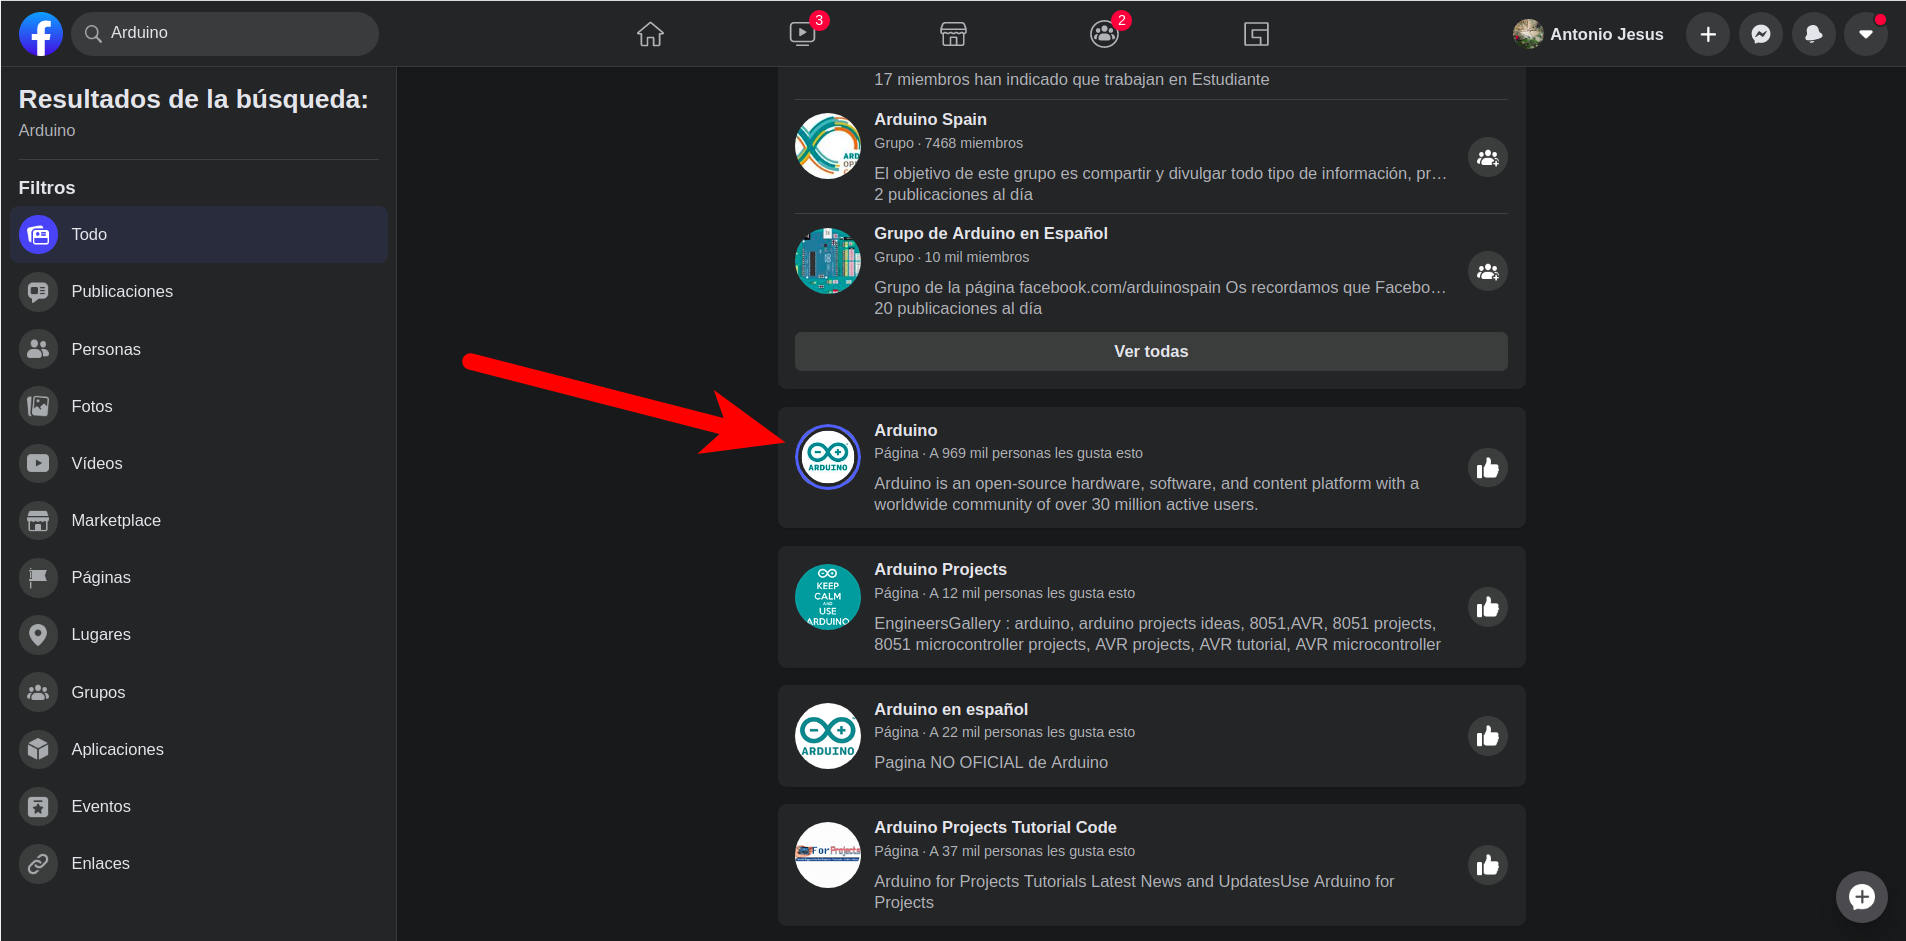
\includegraphics[width=0.7\textwidth]{images/capturas/seleccionusuario.png}
		\caption{Primero: elegimos usuario.}
		\label{fig:seluser}	
\end{figure}
Una vez que sabemos el usuario, nos aparecerá los álbumes de fotografiás que este tiene y elegiremos uno. 
\begin{figure}[H]
	\centering
	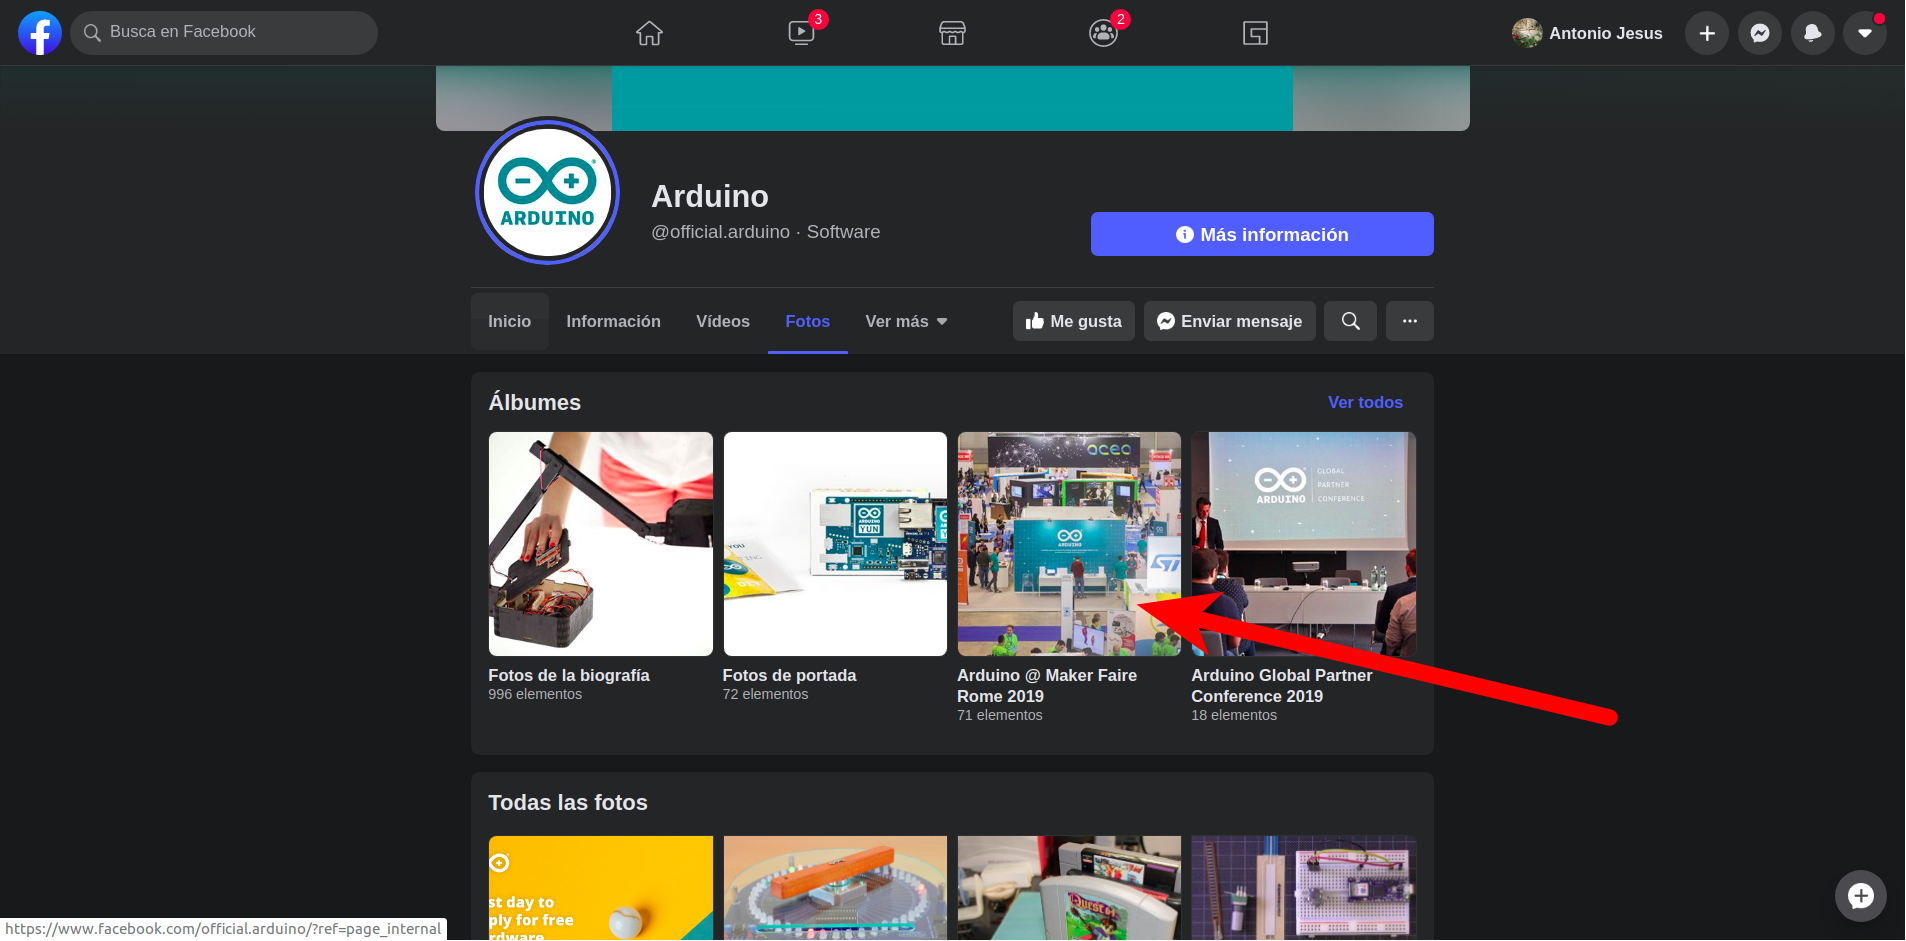
\includegraphics[width=0.7\textwidth]{images/capturas/seleccionAlbun.png}
	\caption{Segundo: elegimos un álbum}
	\label{fig:selalbum}
\end{figure}
Y ya dentro de un álbum podremos elegir una fotografiá. 
\begin{figure}[H]	
	\centering
	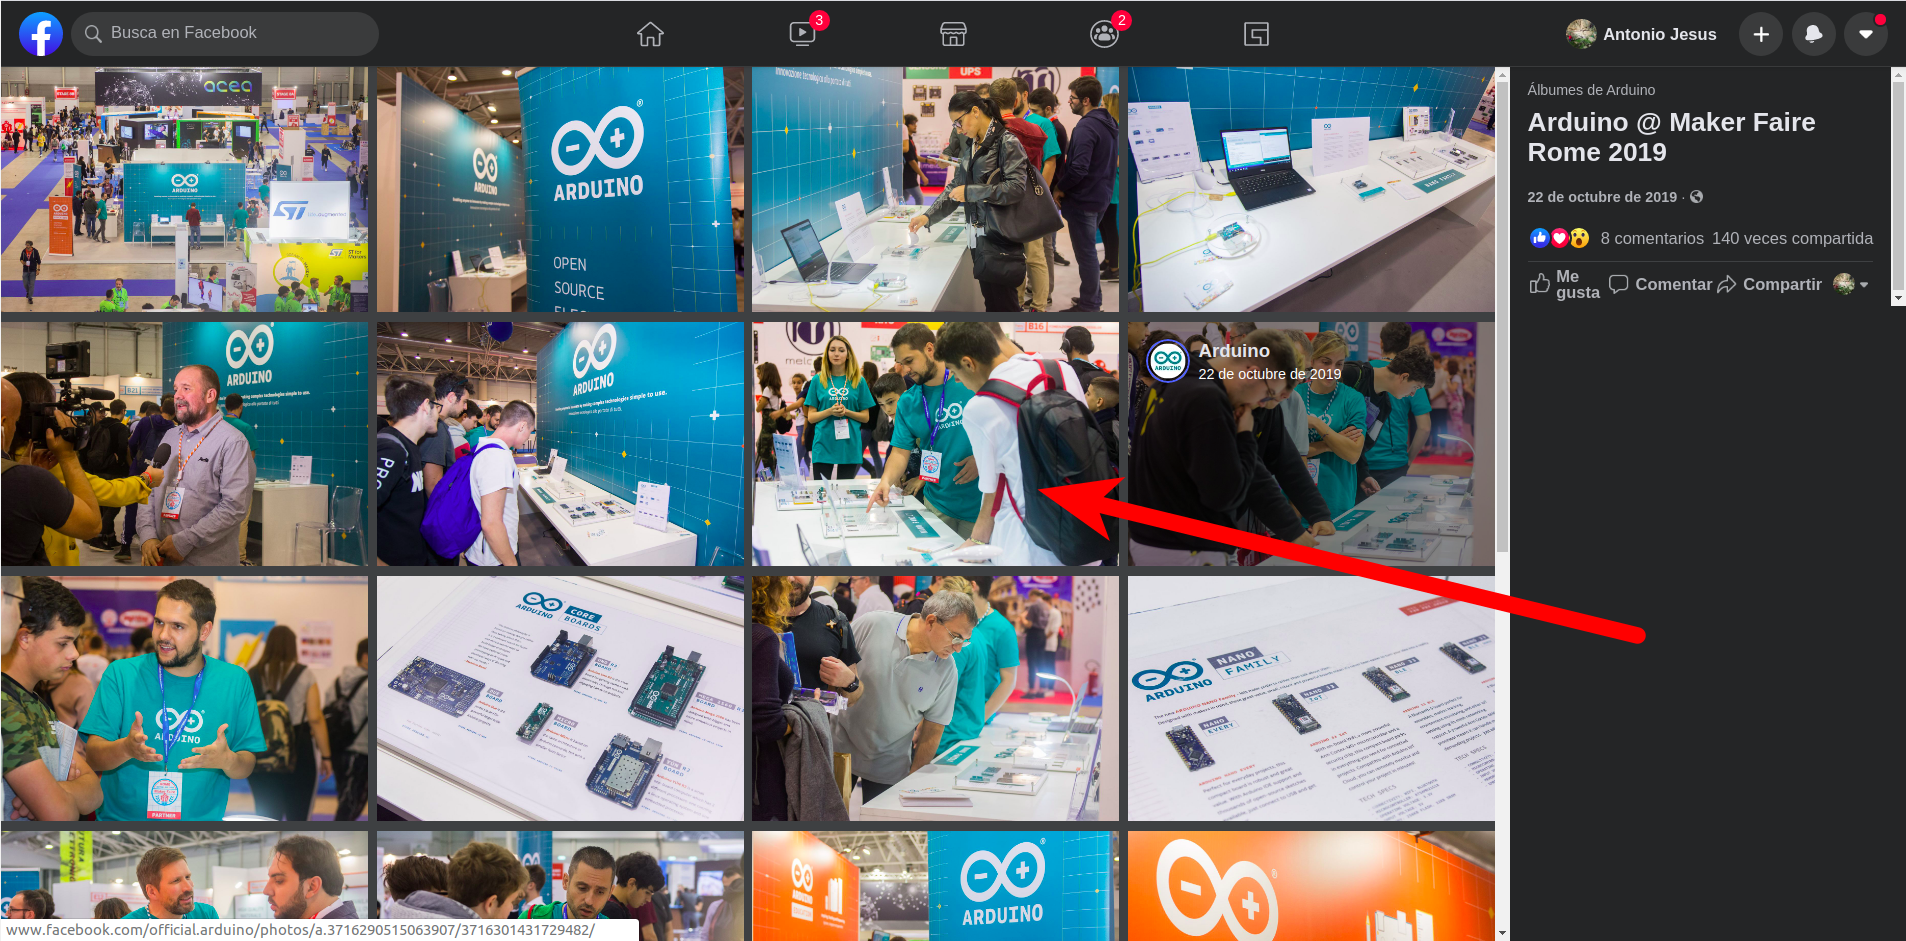
\includegraphics[width=0.7\textwidth]{images/capturas/seleccionImagen.png}
	\caption{Tercero: elegimos la imagen}
	\label{fig:selimagen}
\end{figure}
Y ya por fin podremos ver la fotografía. 
\begin{figure}[H]
	\centering
	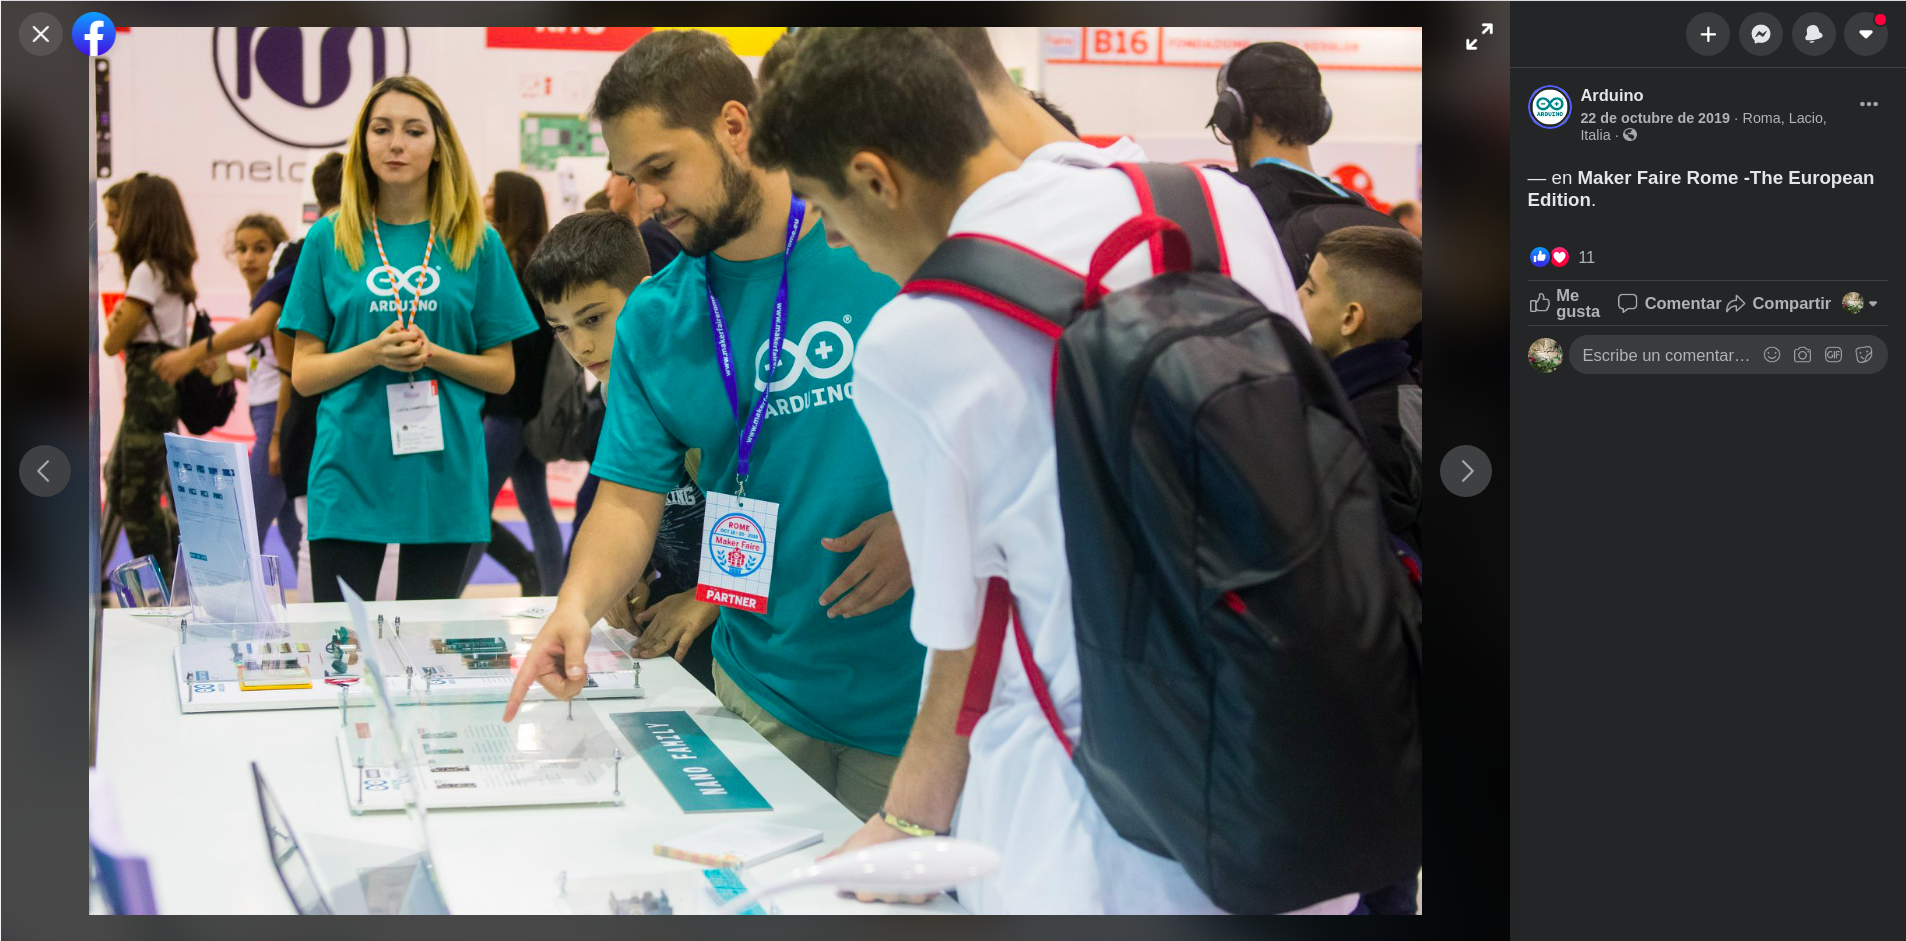
\includegraphics[width=0.7\textwidth]{images/capturas/imagen.png}
	\caption{Cuarto: vemos la imagen}
	\label{fig:imagen}	
\end{figure}
Aunque para llegar a aquí hay casi infinitas formas, nosotros vamos a realizar el IFML de esta. 
\begin{figure}[H]
	\centering
	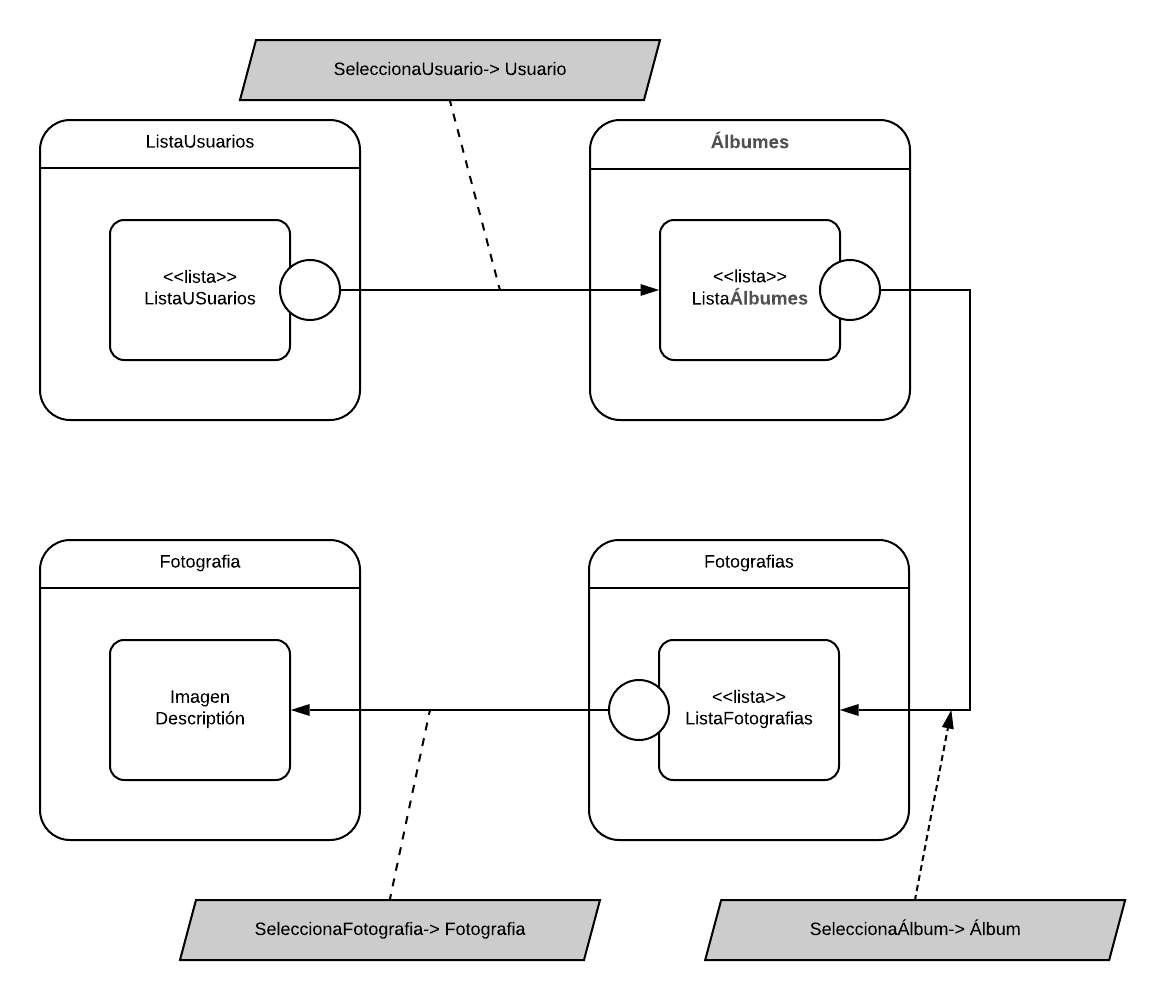
\includegraphics[width=0.9\textwidth]{images/ifml/seleccionProducto.png}
	\caption{IFML de visualización de una imagen. }
	\label{fig:ifmlimagen}	
\end{figure}
En la Figura \ref{fig:ifmlimagen} podemos ver los pasos que debería seguir un usuario para llegar a ver una imagen, que son los mismos que hemos mostrados en las capturas de la aplicación web. 
\subsection{Crear una publicación}
El siguiente ejemplo que vamos a ver seria una de las cosas mas comunes que sea hacen en Facebook, crear una publicación. 
\begin{figure}[H]
	\centering
	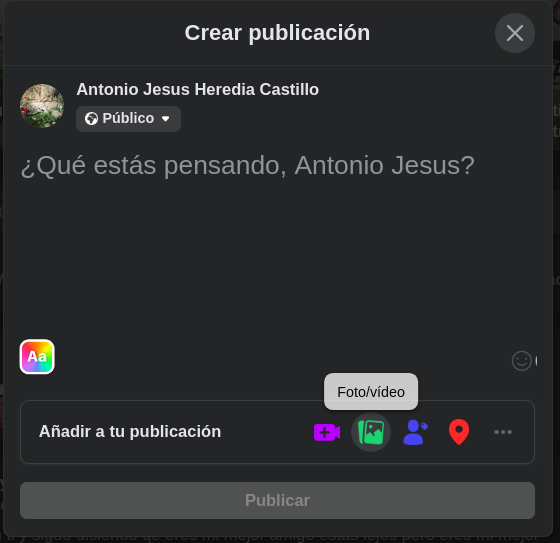
\includegraphics[width=0.5\textwidth]{images/capturas/escribirComentario.png}
	\caption{Creación de una publicación. }
	\label{fig:post}	
\end{figure}
Aunque dentro de una publicación puedes añadir muchas cosas, como el proceso es el mismo yo lo he simplificado en tres apartados. El primero, el mas obvio, el texto del comentario, después la posibilidad de añadir alguna imagen y por ultimo etiquetar a gente en ella. \\
Esto se puede ver mejor en el IFML de esta acción:
\begin{figure}[H]
	\centering
	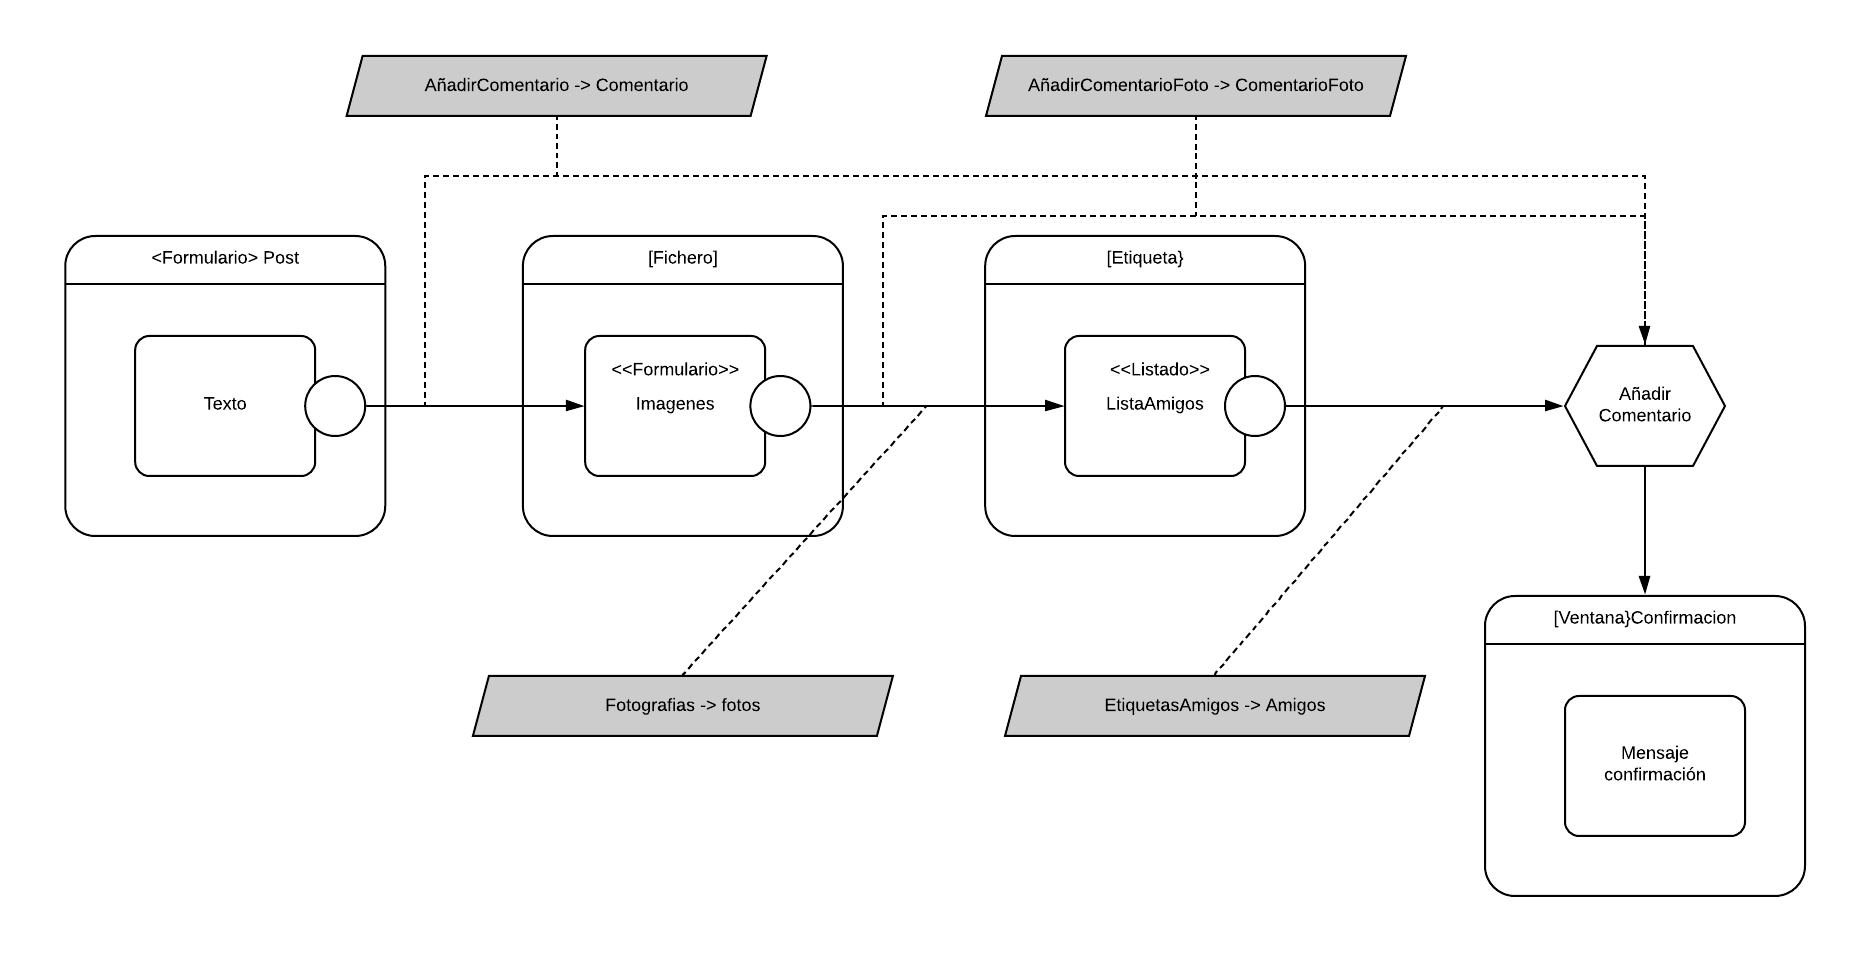
\includegraphics[width=0.9\textwidth]{images/ifml/aniadirImagen.png}
	\caption{IFML de crear una publicación. }
	\label{fig:ifmlpublicacion}	
\end{figure}
En la Figura \ref{fig:ifmlpublicacion} podemos ver como, existe varios flujos de trabajo. Esto se debe a que, puede ver publicaciones que no lleven imagen o publicaciones sin personas etiquetadas. Aunque siempre nos llevara a \textbf{añadir comentario} y finalmente nos muestra una venta indicando que la publicación se ha creado correctamente. 
\subsection{Enviar un mensaje}
Por ultimo vamos a ver los pasos que se deberán seguir para enviar un mensaje a una persona. Primero, como es lógico, tendremos que elegir a quien le vamos ha hablar. 
\begin{figure}[H]
	\centering
	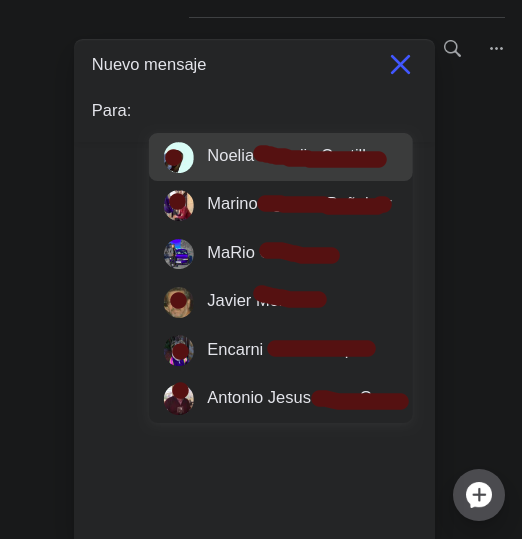
\includegraphics[width=0.3\textwidth]{images/capturas/elegirMensajero.png}
	\caption{Elegimos un usuario con el que hablar. }
	\label{fig:mensajero}	
\end{figure}
Ademas de añadir nuestro mensaje tendremos opciones como añadir una imagen.
\begin{figure}[H]
	\centering
	
\includegraphics[width=0.3\textwidth]{images/capturas/escribirMensaje.png}
	\caption{Escribimos el mensaje.}
	\label{fig:mensaje}	
\end{figure}
En la Figura \ref{fig:ifmlmensaje} podemos cual sera el flujo de enviar un mensaje. Lo primero que realizamos es elegir al usuario que queremos enviar el mensaje, después escribimos y por ultimo podemos añadir una imagen al mensaje. Como he hecho en el ejemplo anterior he simplificado, ya que se puede enviar casi infinitas cosas. 
\begin{figure}[H]
	\centering
	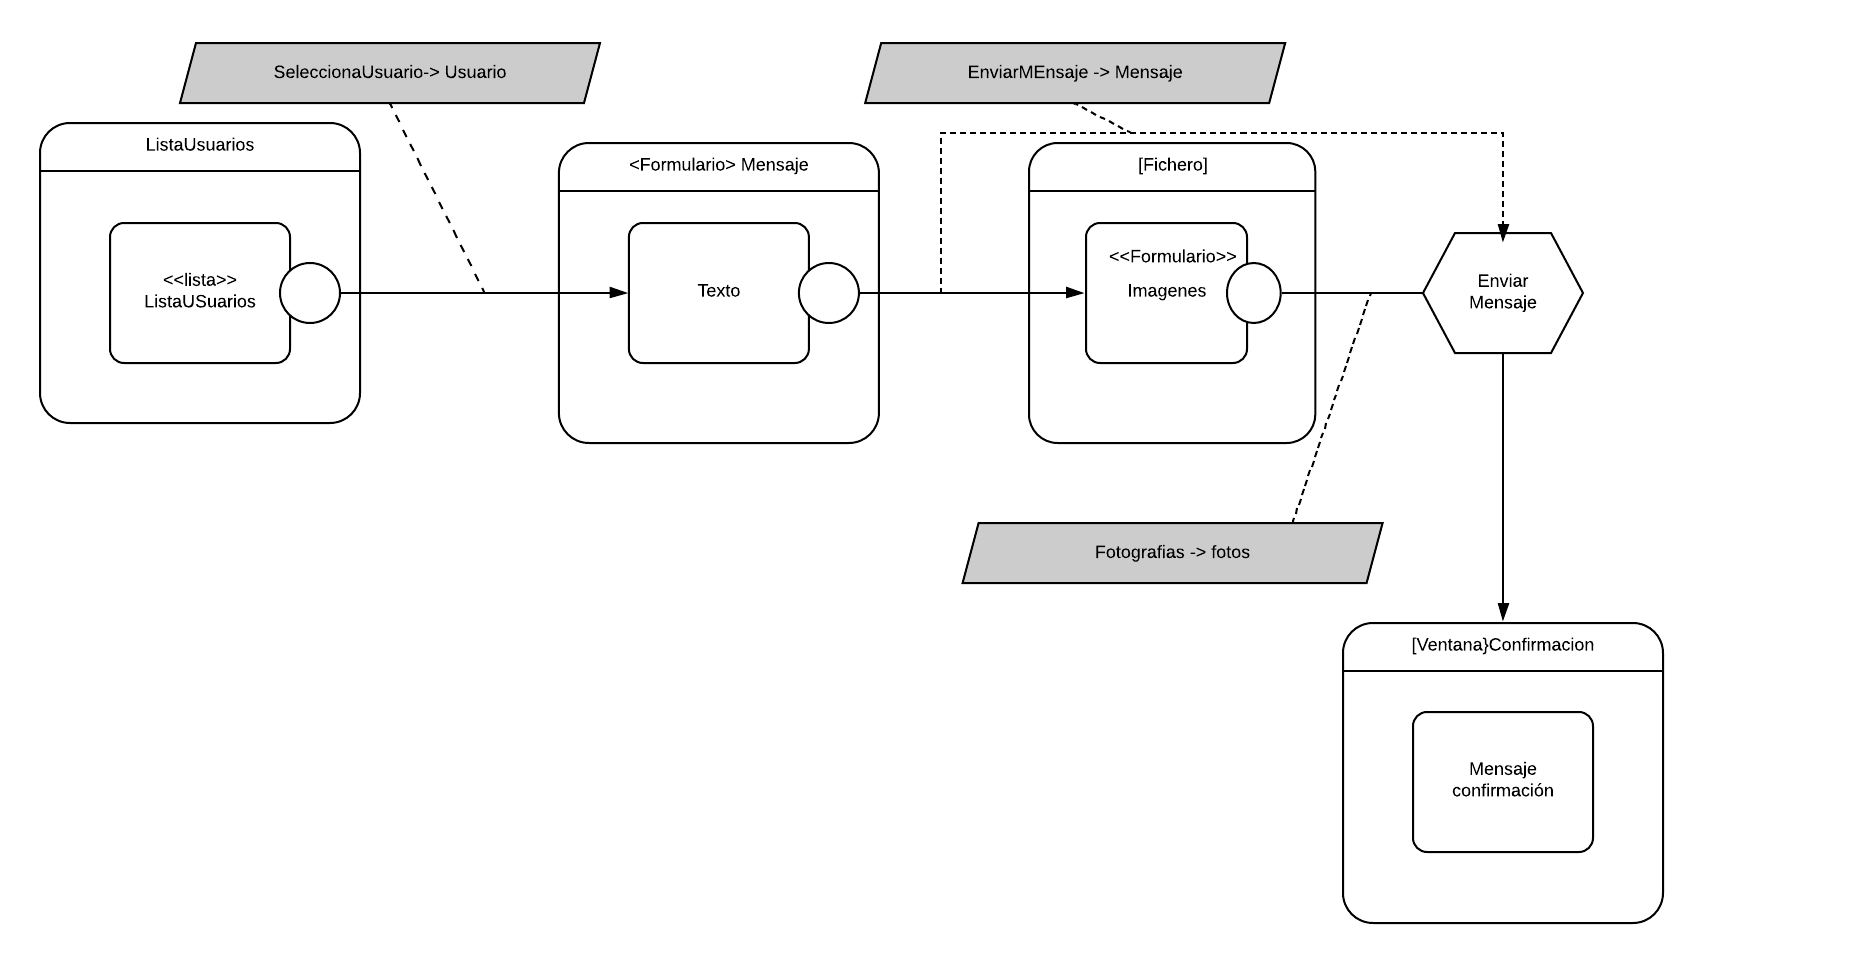
\includegraphics[width=0.9\textwidth]{images/ifml/enviarMensaje.png}
	\caption{IFML de crear una publicación. }
	\label{fig:ifmlmensaje}	
\end{figure}
\section{Ejercicio 2: Alternativas a jQuery}
Para la ampliación de un tema relacionado con la asignatura he elegido dar a conocer las distintas alternativas a jQuery. Explicare algunas de estas alternativas y realizare comparaciones para ver cual puede sernos mas util para nuestro proyecto.
\subsection{zepto.js}
El primero  que vamos a ver es zepto. 
\begin{figure}[H]
	\centering
	
\includegraphics[width=0.5\textwidth]{images/zepto.png}
\end{figure}
Consigue lo mismo que jQuery pero usando mucho menos espacio y tiempo, lo cual lo hace muy útil para evitar sobrecargar las conexiones. Fue ideada para usar en dispositivos móviles y navegadores modernos. Aunque la siguiente alternativa que vamos a ver gana a los dos en ese aspecto.
\subsection{Cash}
 El siguiente sera \href{https://github.com/fabiospampinato/cash}{Cash}. 

\begin{figure}[H]
	\centering
	
\includegraphics[width=0.3\textwidth]{images/cash.png}
\end{figure}
Al igual que zepto una sintaxis similar que jQuery para manipular el DOM, pero donde gana terreno es en su tamaño, donde podemos conseguir hasta ganancias del $76\%$.\\\\
\begin{table}[H]
	\centering
\begin{tabular}{|c|c|c|}
	\hline 
	\textbf{Tamaño} & \textbf{Cash} & \textbf{jQuery Slim} \\ 
	\hline 
	\textbf{Sin minificar} & 34.9 KB & 227 KB \\ 
	\hline 
	\textbf{Minificado} & 15.3 KB & 71 KB \\ 
	\hline 
	\textbf{Minificado y Gzipped} & 5.7 KB & 24.4 KB \\ 
	\hline 
\end{tabular} 
\end{table}

Uno de sus problemas frente a jQuerey es que no es soportado por navegadores antiguos. Pero también tiene sus ventajas como que podemos usar el tipado de TypeScript. \\
\\
A continuación podemos ver un ejemplo de una función usando Cash, donde añadimos un footer al html, que como vemos es igual que con jQuery. 

\lstset{
	language=JavaScript,
	backgroundcolor=\color{white},
	extendedchars=true,
	basicstyle=\footnotesize\ttfamily,
	showstringspaces=false,
	showspaces=false,
	numbers=left,
	numberstyle=\footnotesize,
	numbersep=9pt,
	tabsize=2,
	breaklines=true,
	showtabs=false,
	captionpos=b
}
\begin{lstlisting}[frame=single]  % Inicia el bloque de código
import $ from "cash-dom";

$(function () {
	$('html').addClass ( 'dom-loaded' );
	$('<footer>Appended with Cash</footer>')
	.appendTo( document.body );
});
\end{lstlisting}
\subsection{Umbrella}
El siguiente que vamos a ver se llama \textbf{Umbrella}.
\begin{figure}[H]
	\centering
	
\includegraphics[width=0.4\textwidth]{images/umbrella.png}
\end{figure}
En este caso Umbrella también esta fuertemente influenciada por jQuery. También nos provee manipulación del DOM, manejo de eventos y un uso amigable de AJAX. Nos trae la mayoría de métodos de jQuery y añade métodos nuevos. También es mucho mas ligero que jQuery (solo 4 KB). Una pequeña diferencia de sintaxis es que cambia el \$() por  u(). Un punto importante seria su buena documentación.
\\
\\
Un ejemplo de helloWorld con Umbrella seria:
\begin{lstlisting}[frame=single]
u("button").on('click', function(){
	alert("Hello world");
});
\end{lstlisting}

\subsection{MooTools}
Ahora vamos a hablar de \textbf{MooTools}.
\begin{figure}[H]
	\centering
	
\includegraphics[width=0.4\textwidth]{images/mootools.png}
\end{figure}
Es una herramienta pensada para programadores experimentados en JavaScript.  Es un framework que intenta implementar JavaScript. Esta enfocado a orientación de objetos. Es modular y extensible, donde el programador es el que elige que modulo quiere usar. Podemos distinguir las siguientes herramientas:
\begin{itemize}
	\item \textbf{Core}: es el nucleo e implementa el concepto de las clases.
	\item \textbf{More}: es la colección oficial de plugins  e incorpora gran cantidad de mejoras.
	\item \textbf{Class}: necesaria para crear instancias de clases de objetos.
	\item \textbf{Element}: Es el que nos permite manejar el DOM.
	\item \textbf{Fx}: nos sirve como base para la animación de elementos.
	\item \textbf{JSON}: modulo par la codificación y decodificación de cadenas en formato JSON.
\end{itemize}
Algunos de estos modulos se complementan entre si. Ademas \textbf{MooTools} es muy utilizado para las aplicaciones de tipo single page. 
\subsection{Ext JS}
Otro gran competidor es \textbf{Ext JS}. Una biblioteca para JS desarrollada por Sencha. 
\begin{figure}[H]
	\centering
	
\includegraphics[width=0.4\textwidth]{images/extjs.jpeg}
\end{figure}
Esta librería nos incluye infinidad de componentes, más de 140 según la propia empresa. Estos componentes van desde los típicos formularios, menús listas hasta cosas mas avanzadas como graficas, arboles y calendarios. El gran inconveniente que tiene es que es una opción de pago, por lo tanto solo he podido hacer uso de una versión de prueba de 30 días que te dan. Si no fuera por ello es una de las alternativas más interesantes a jQuery.  Lo bueno es que tiene una versión \textbf{GLP}, aunque su curva de aprendizaje es mucho mayor.

\end{document}
	